%%%%%%%%
\documentclass [11pt, a4paper, leqno] {article}
\usepackage [polish] {babel}
\usepackage {polski}
\usepackage [utf8] {inputenc}
\usepackage [T1] {fontenc}
\usepackage {indentfirst}
\usepackage {setspace}
\usepackage {amstext}
\usepackage {amsfonts}
\usepackage {graphicx}
\DeclareGraphicsExtensions{.png}
\setstretch {1.15} %interlinia
\frenchspacing
\renewcommand {\thesection} {\arabic{section}.}
\renewcommand {\thesubsection} {\arabic{section}. \arabic{subsection}.}
\renewcommand {\thesubsubsection} {\arabic{section}. \arabic{subsection}. \arabic{subsubsection}.}
\textheight 610pt
\makeatletter
\renewcommand\@biblabel[1]{#1}
\makeatother
\usepackage[a4paper,left=3.8cm,right=3.8cm,top=3.3cm,bottom=3cm]{geometry}
%%%%%%%%

\begin{document}
% STRONA TYTUŁOWA

\begin{center}
  \thispagestyle{empty} %usunięcie numeracji
  {\large Studencka Pracownia Inżynierii Oprogramowania} \\ [0.5cm]
	{\large Instytut Informatyki Uniwersytetu Wrocławskiego} \\ [6.0cm]

  {\large Rafał Florczak, Dominik Rabij} \\ [1.5cm]

	{\huge Dokumentacja oprogramowania} \\ [0.5cm]
  {\huge RECEPCJONISTA} \\ [1.5cm]

  {\large Plan bazy danych} \\ [0.5cm]

  \vfill
  
  {\large Wrocław, \today} \\ [0.5cm]

  {\large Wersja 0.2}
\end{center}

\newpage

% TABELKA WERSJI

\textit{Tabela 0.} Historia zmian dokonanych w dokumencie

\begin{center}
  \begin{tabular}{| l | l | l | l |}
    \hline
    \multicolumn{1}{|c|}{Data} & 
    \multicolumn{1}{|c|}{Numer wersji} &  
    \multicolumn{1}{|c|}{Opis} &
    \multicolumn{1}{|c|}{Autor} \\ \hline \hline
    2015-12-16 & 0.1 & Utworzenie dokumentu & Rafał Florczak \\ \hline
    2016-01-13 & 0.2 & Naniesienie poprawek & Rafał Florczak \\ \hline
  \end{tabular}
\end{center}

\medskip

\tableofcontents

\newpage

\section{Wprowadzenie}

\subsection{Cel dokumentu}
\noindent
Celem niniejszego dokumentu jest przedstawienie rozwiązań wybranych przez projektantów bazy danych. Dalej przedstawiono wybrany system zarządzania bazą danych oraz schemat relacji. Są one ważne, jeśli chodzi o sprawne działanie Recepcjonisty.

Dokument jest przeznaczony dla programistów oraz osób, które będą zajmowały się utrzymaniem oprogramowania w przyszłości.

\section{Baza danych}
\subsection{System zarządzania bazą danych}
\noindent
Do przechowywania i nadzoru nad zasobami bazy danych wybrany został system PostgreSQL, ponieważ jest on bezpłatny, stabilny, szybki i popularny, a jego kod jest dostępny publicznie.

\subsection{Schemat bazy danych}


\begin{center}
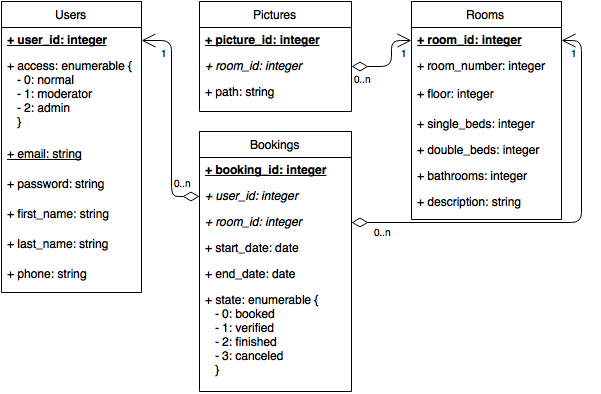
\includegraphics[scale=0.7]{recepcjonistadb}
\textit{Rysunek 1.} Schemat bazy danych
\end{center}

\newpage
\noindent
Opis notacji zastosowanej na rys. 1: 
\begin{itemize}
  \item podkreślenie --- klucz relacji,
  \item pogrubienie --- klucz główny relacji,
  \item kursywa --- klucz obcy,
  \item $\Diamond$---------> --- relacja jeden-do-wielu.
\end{itemize}

\subsubsection{Użytkownicy (\textit{users})}
\noindent
Tabela przechowuje informacje o wszystkich użytkownikach Recepcjonisty --- zarówno o klientach, jak i  jego obsłudze. Pole \textit{access} określa uprawnienia danego użytkownika.

\subsubsection{Rezerwacje (\textit{bookings})}
\noindent
Relacja zawiera informacje o rezerwacjach (także tych zakończonych i anulowanych).

\subsubsection{Pokoje (\textit{rooms})}
\noindent
Tabela przedstawia dane o pokojach w hotelu. Informacje o liczbie łóżek zostały rozdzielone na dwa odrębne pola --- \textit{$single_{-}beds$} oraz \textit{$double_{-}beds$} oznaczające odpowiednio liczbę łóżek jednoosobowych i dwuosobowych.

\subsubsection{Zdjęcia (\textit{pictures})}
\noindent
Relacja przechowuje nazwy bezwzględne plików ze zdjęciami poszczególnych pokojów.


\end{document}